\section{Momentum with System Heterogeneity}
\label{sec:autonomous}

\subsection{Autonomous Multistage FedGM}

For a simplified abstraction of real world settings, most FL algorithms make the assumption that, all clients synchronize with the same global model and they conduct identical number of local updates at any given round. Though the assumption has been adopted in most existing works \citep{McMahan2017FedAvg,Hsu2019MeasuringTE,Li20FedProx,karimireddy2020scaffold,reddi2020adaptive,bao2022doubly, wang22adaptive}, it rarely holds in reality.

In light of the limitations of existing works, we propose a general framework called Autonomous Multistage FedGM that enables the following three features, i.e. \textbf{heterogeneous local computing}, \textbf{asynchronous aggregation}, and \textbf{flexible client participation}, which is formalized in Algorithm \ref{alg:autonomous_fedgm}. 

Autonomous Multistage FedGM could effectively mitigate straggler effect and poor convergence issue in highly heterogeneous cross-device deployments. We leave a more detailed discussion of Algorithm \ref{alg:autonomous_fedgm} to Appendix \ref{sec:autonomous_multistage} due to space limit.

Specifically, in Autonomous Multistage FedGM, the client decides when to participate in the training, and idling between rounds or even completely unavailable are both allowed. Once it decides to participate at round $t$, it retrieves current global model $x_\mu$ from the server and conduct $K_{t,i}$ local steps to update to $x^i_{\mu,K_{t,i}}$. Note in vanilla FedAvg, $K_{t,i}=K$ for any $i$ and $t$. In contrast, we allow $K_{t,i}$ to be time-varying and device-dependent. The client then normalizes the model update by $K_{t,i}$ to avoid model biased towards clients with more local updates. Concurrently, the server collects the model updates from the clients. As every client may participate in training at a different round, the collected model update $\Delta_{t-\tau_{t,i}}^i$ may be from a historic timestamp, i.e. $\tau_{t,i}$ away from current time $t$. The server triggers global update whenever it collects $m$ model updates and we denote the set of $m$ responsive clients as $\mathcal{S}_t$. The global update is same as multistage FedGM (i.e. Lines 11-13). Note that server optimization is concurrent with clients, i.e., the global update happens whenever $m$ model updates are collected, regardless of whether there are still some clients conducting local computation, thus ensuring there is no straggler.


Autonomous multistage FedGM, i.e. Algorithm \ref{alg:autonomous_fedgm}, will recover multistage FedGM, i.e. Algorithm \ref{multistage_FedGM_algorithm}, if we set $K_{t,i}=K$ and $\tau_{t,i}=0$ for $\forall t, i$. Please note that varying $K_{t,i}$ and nonzero $\tau_{t,i}$ bring nontrivial extra complexity to the theoretical analysis as can be seen in our proof.

\begin{algorithm2e}[tb]
\SetAlgoVlined
\KwIn{Same as Algorithm \ref{multistage_FedGM_algorithm}}
\SetAlgoLined
\For{$s\in\{1,...,S\}$}
{
\For{$t $ \text{in stage} $s$}
{   
    \colorbox{babyblueeyes}{\textbf{At Each Client (Concurrently)}}
    
    Once decided to participate in the training, retrieve $x_\mu$ from the server and its timestamp, set $x_{\mu,0}^i=x_\mu$.

    Select a number of local steps $K_{t,i}$, which is time-varying and device-dependent.

    $\Delta_\mu^i=\textbf{LocalOPT}\left(i,\eta_l,K_{t,i},x_\mu\right)$

    Normalize and send $\Delta_\mu^i=\frac{\Delta_\mu^i}{K_{t,i}}$
    

    \colorbox{babyblueeyes}{\textbf{At Server (Concurrently)}}
    
    Collect $m$ local updates $\{\Delta_{t-\tau_{t,i}}^i, i\in\mathcal{S}_t\}$ returned from the clients to form set $\mathcal{S}_t$, where $\tau_{t,i}$ is the random delay of the client $i$'s local update, $i\in\mathcal{S}_t$

    Aggregate $\Delta_t=\frac{1}{\lvert\mathcal{S}_t\rvert}\sum_{i\in \mathcal{S}_t}\Delta_{t-\tau_{t,i}}^i$

    $d_{t+1}=(1-\beta_s)\Delta_{t}+\beta_s d_{t}$

    $h_{t+1}=(1-\nu_s)\Delta_{t}+\nu_s d_{t+1}$
        
    Update $x_{t+1}=x_t-\eta_s h_{t+1}$

}
}
return $x_T$
\caption{\colorbox{babyblueeyes}{Autonomous Multistage FedGM}}
\label{alg:autonomous_fedgm}
\end{algorithm2e}


\iffalse

\subsection{Ubiquitous System Heterogeneity}

For a simplified abstraction of real world settings, most FL algorithms make the assumption that, all clients initialize with the same global model and they conduct identical number of local updates at any given round.

More formally, we could observe from LocalOPT (Algorithm \ref{alg:localopt}) that the following assumptions have been made, (a) \textit{Homogeneous Local Updates} all participating clients would do local gradient descent for $K$ steps; (b) \textit{Uniform Client Participation} each client would participate in a given communication round uniformly according to a given distribution that is independent across rounds; (c) \textit{Synchronous Local Clients} all participating clients always initialize at $x_t$, i.e., the global model at current timestamp. 



Though these three assumptions have been adopted in most existing works \citep{McMahan2017FedAvg,Hsu2019MeasuringTE,Li20FedProx,karimireddy2020scaffold,reddi2020adaptive,wang22adaptive}, each of these assumptions rarely holds in reality. Due to unavoidable \textbf{heterogeneous client capability}, and \textbf{unpredictable availability}, enforcing identical local epochs and synchrony would incur straggler effect and unnecessary energy waste \citep{Kairouz21AdvancesProblems}. Therefore, realistic FL system is more economical to allow different local epochs and \textbf{asynchronous aggregation}.


When studying client heterogeneity and the resulting client drift, most works focus explicitly on data heterogeneity \citep{Li2020Fed-Non-IID,yang2021achieving}, while ignoring the equally ubiquitous system heterogeneity, which casts doubt on the applicability of the corresponding algorithms in practice.


\begin{algorithm2e}[tb]
\SetAlgoVlined
\KwIn{Same as Algorithm \ref{multistage_FedGM_algorithm}}
\SetAlgoLined
\For{$s\in\{1,...,S\}$}
{
\For{$t $ \text{in stage} $s$}
{   
    \colorbox{babyblueeyes}{\textbf{At Each Client (Concurrently)}}
    
    Once decided to participate in the training, retrieve $x_\mu$ from the server and its timestamp, set $x_{\mu,0}^i=x_\mu$.

    Select a number of local steps $K_{t,i}$, which is time-varying and device-dependent.

    $\Delta_\mu^i=\textbf{LocalOPT}\left(i,\eta_l,K_{t,i},x_\mu\right)$

    Normalize and send $\Delta_\mu^i=\frac{\Delta_\mu^i}{K_{t,i}}$
    

    \colorbox{babyblueeyes}{\textbf{At Server (Concurrently)}}
    
    Collect $m$ local updates $\{\Delta_{t-\tau_{t,i}}^i, i\in\mathcal{S}_t\}$ returned from the clients to form set $\mathcal{S}_t$, where $\tau_{t,i}$ is the random delay of the client $i$'s local update, $i\in\mathcal{S}_t$

    Aggregate $\Delta_t=\frac{1}{\lvert\mathcal{S}_t\rvert}\sum_{i\in \mathcal{S}_t}\Delta_{t-\tau_{t,i}}^i$

    $d_{t+1}=(1-\beta_s)\Delta_{t}+\beta_s d_{t}$

    $h_{t+1}=(1-\nu_s)\Delta_{t}+\nu_s d_{t+1}$
        
    Update $x_{t+1}=x_t-\eta_s h_{t+1}$

}
}
return $x_T$
\caption{\colorbox{babyblueeyes}{Autonomous Multistage FedGM}}
\label{alg:autonomous_fedgm}
\end{algorithm2e}

\subsection{Autonomous Multistage FedGM}

In light of the limitations of existing works, we aim to propose a general framework that enables all three features, i.e. \textbf{heterogeneous local computing}, \textbf{asynchronous aggregation}, and \textbf{flexible client participation}, which is formalized in Algorithm \ref{alg:autonomous_fedgm}.

Specifically, in Autonomous Multistage FedGM, the client decides when to participate in the training, and idling between rounds or even completely unavailable are both allowed. Once it decides to participate at round $t$, it retrieves current global model $x_\mu$ from the server and initializes $x_{\mu,0}^i=x_\mu$ locally, and conduct $K_{t,i}$ local steps to update from $x_{\mu,0}^i$ to $x^i_{\mu,K_{t,i}}$. Note in vanilla FedAvg, $K_{t,i}=K$ for any $i$ and $t$. In contrast, we allow $K_{t,i}$ to be time-varying and device-dependent. The client then normalizes the model update by $K_{t,i}$, i.e. $\Delta_\mu^i=\frac{x_{\mu,0}^i-x_{\mu,K_{t,i}}^i}{K_{t,i}}$, to avoid model biased towards clients with more local updates. Concurrently, the server collects the model updates from the clients. As every client may participate in training at a different round, the collected model update $\Delta_{t-\tau_{t,i}}^i$ may be from a historic timestamp, i.e. $\tau_{t,i}$ away from current time $t$. If we set the random delay $\tau_{t,i}=0$, it would be ordinary synchronous aggregation. The server triggers global update whenever it collects $m$ model updates and we denote the set of $m$ responsive clients as $\mathcal{S}_t$. The global update is same as multistage FedGM (i.e. Lines 11-13). Note that server optimization is concurrent with clients, i.e., the global update happens whenever $m$ model updates are collected, regardless of whether there are still some clients conducting local computation, thus ensuring there is no straggler.


Autonomous multistage FedGM will recover multistage FedGM, i.e. Algorithm \ref{multistage_FedGM_algorithm}, if we set $K_{t,i}=K$ and $\tau_{t,i}=0$ for $\forall t, i$. Please note that varying $K_{t,i}$ and nonzero $\tau_{t,i}$ bring nontrivial extra complexity to the theoretical analysis as can be seen in our proof.

\fi


\begin{figure}[h]

\centering
\subfigure{

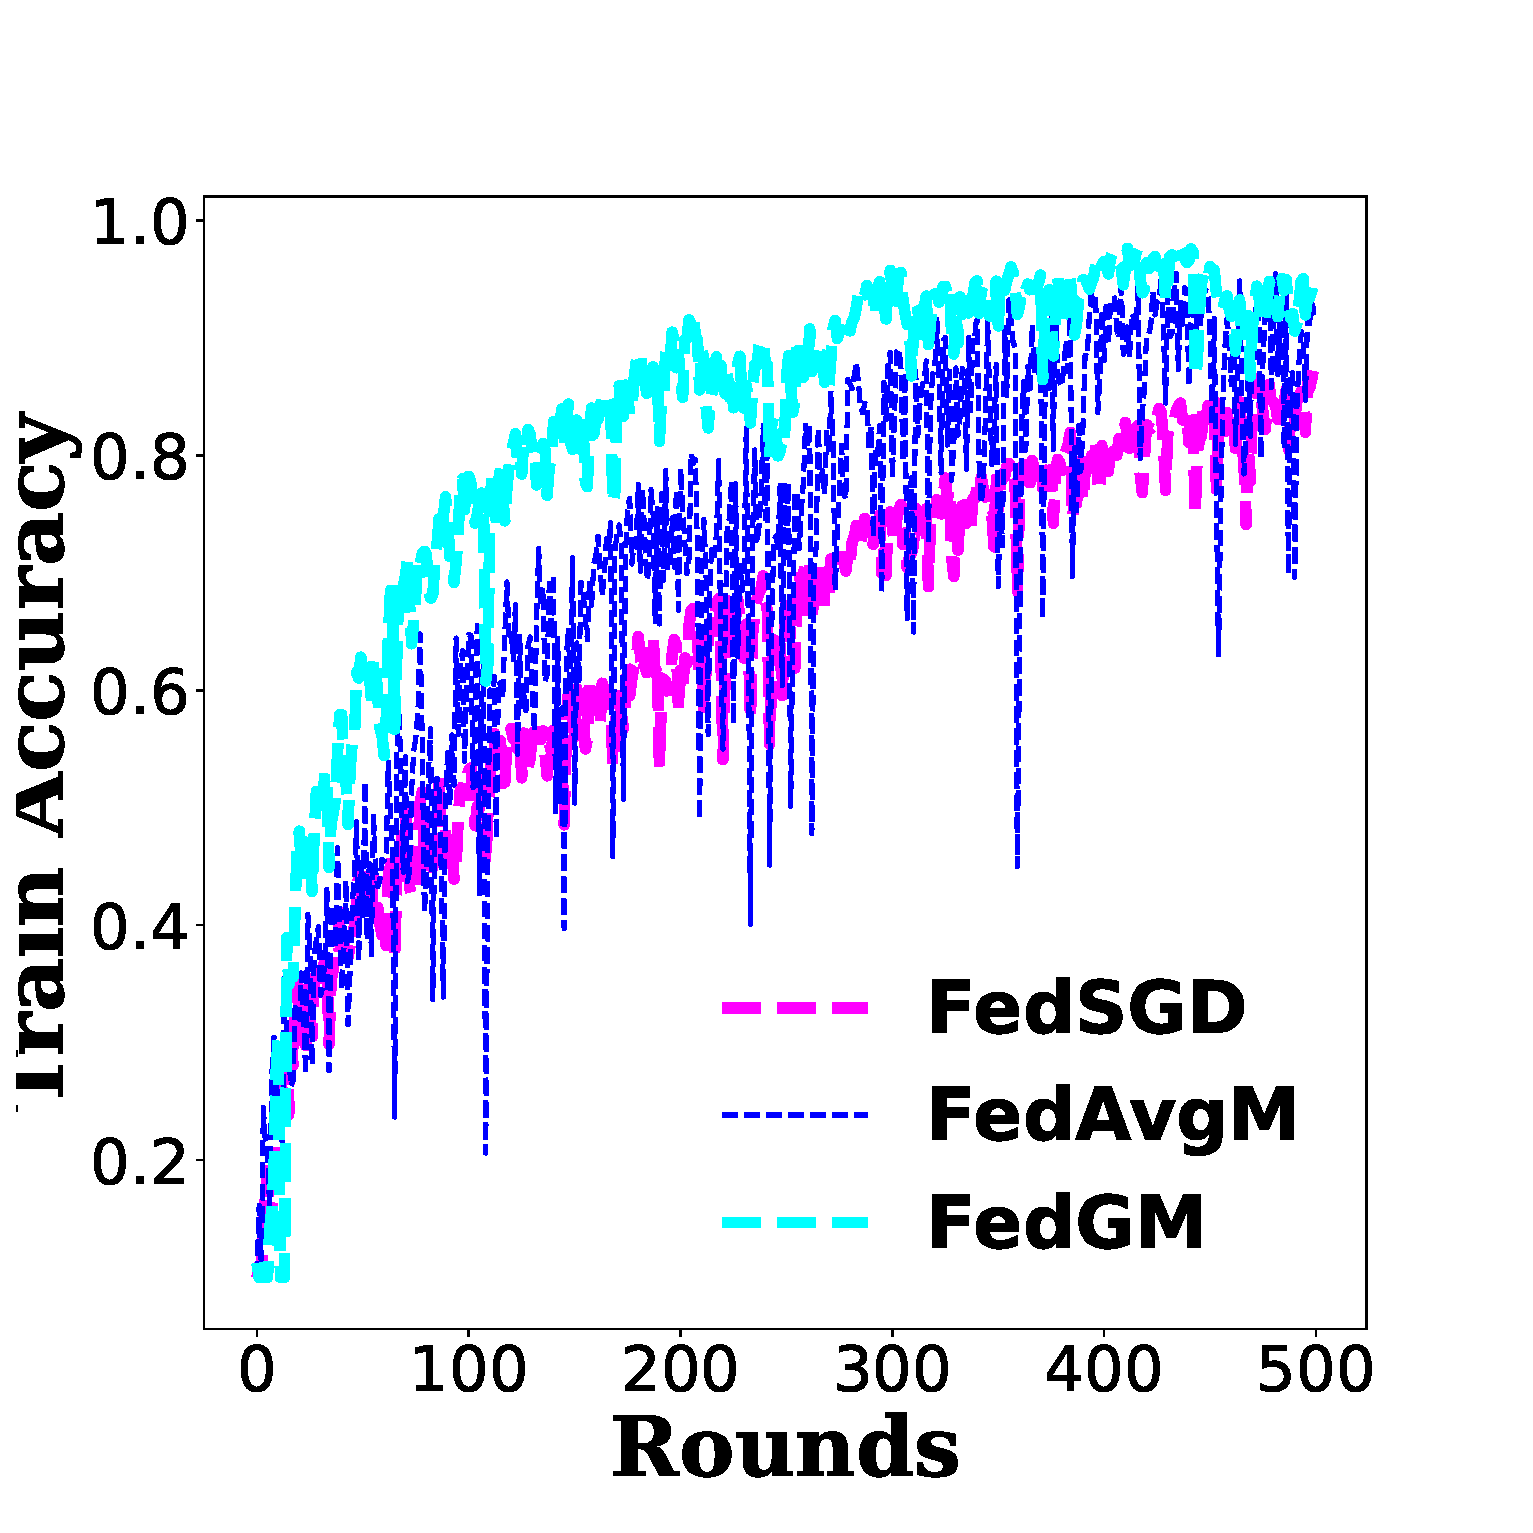
\includegraphics[width=.21\textwidth]{figs/resnet_cifar10_train.eps}
\label{subfig:resnet_cifar10_train}
}
\hspace{-2pt}
\subfigure{
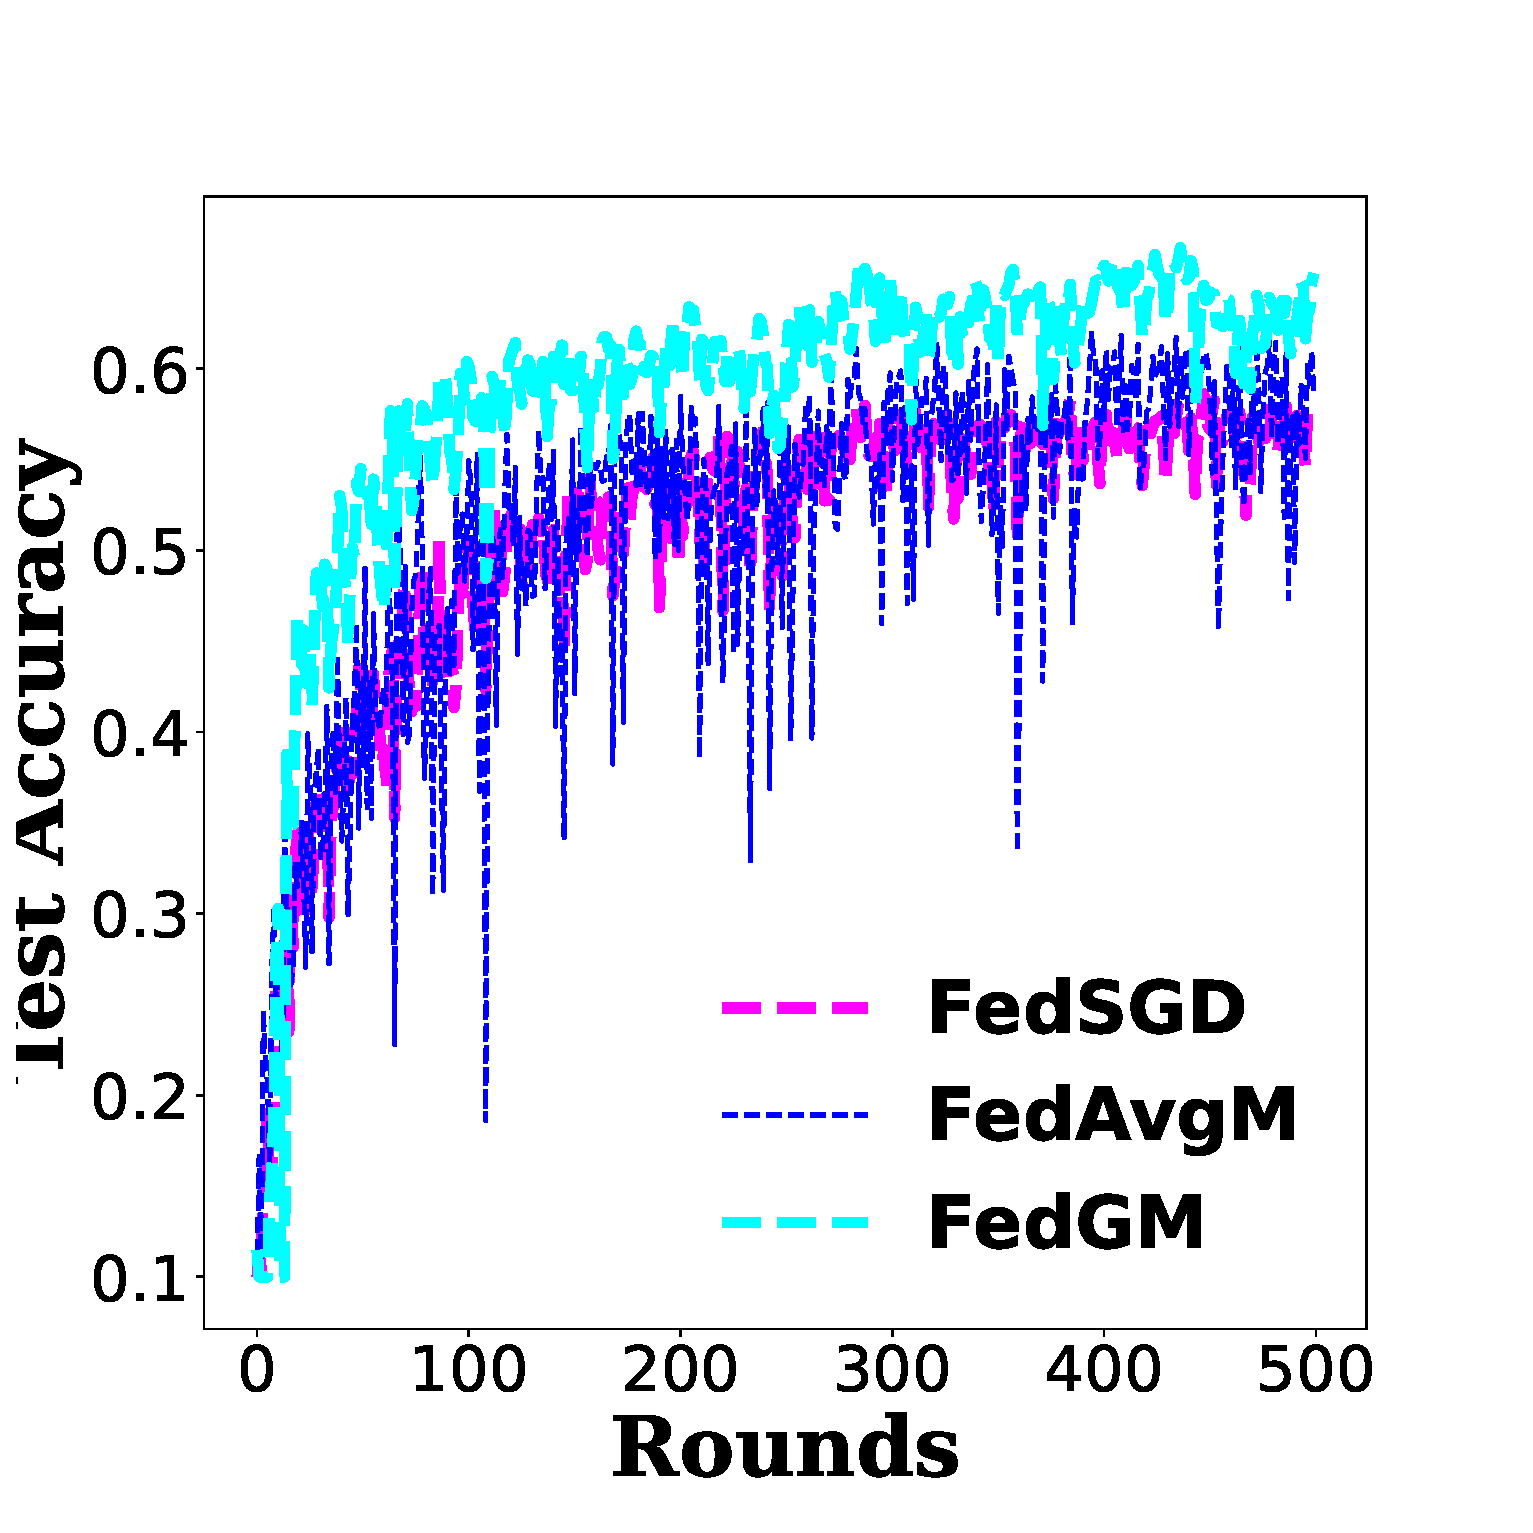
\includegraphics[width=.21\textwidth]{figs/resnet_cifar10_test.eps}
\label{subfig:resnet_cifar10_test}
}
\hspace{-2pt}
\subfigure{
\hspace{0pt}
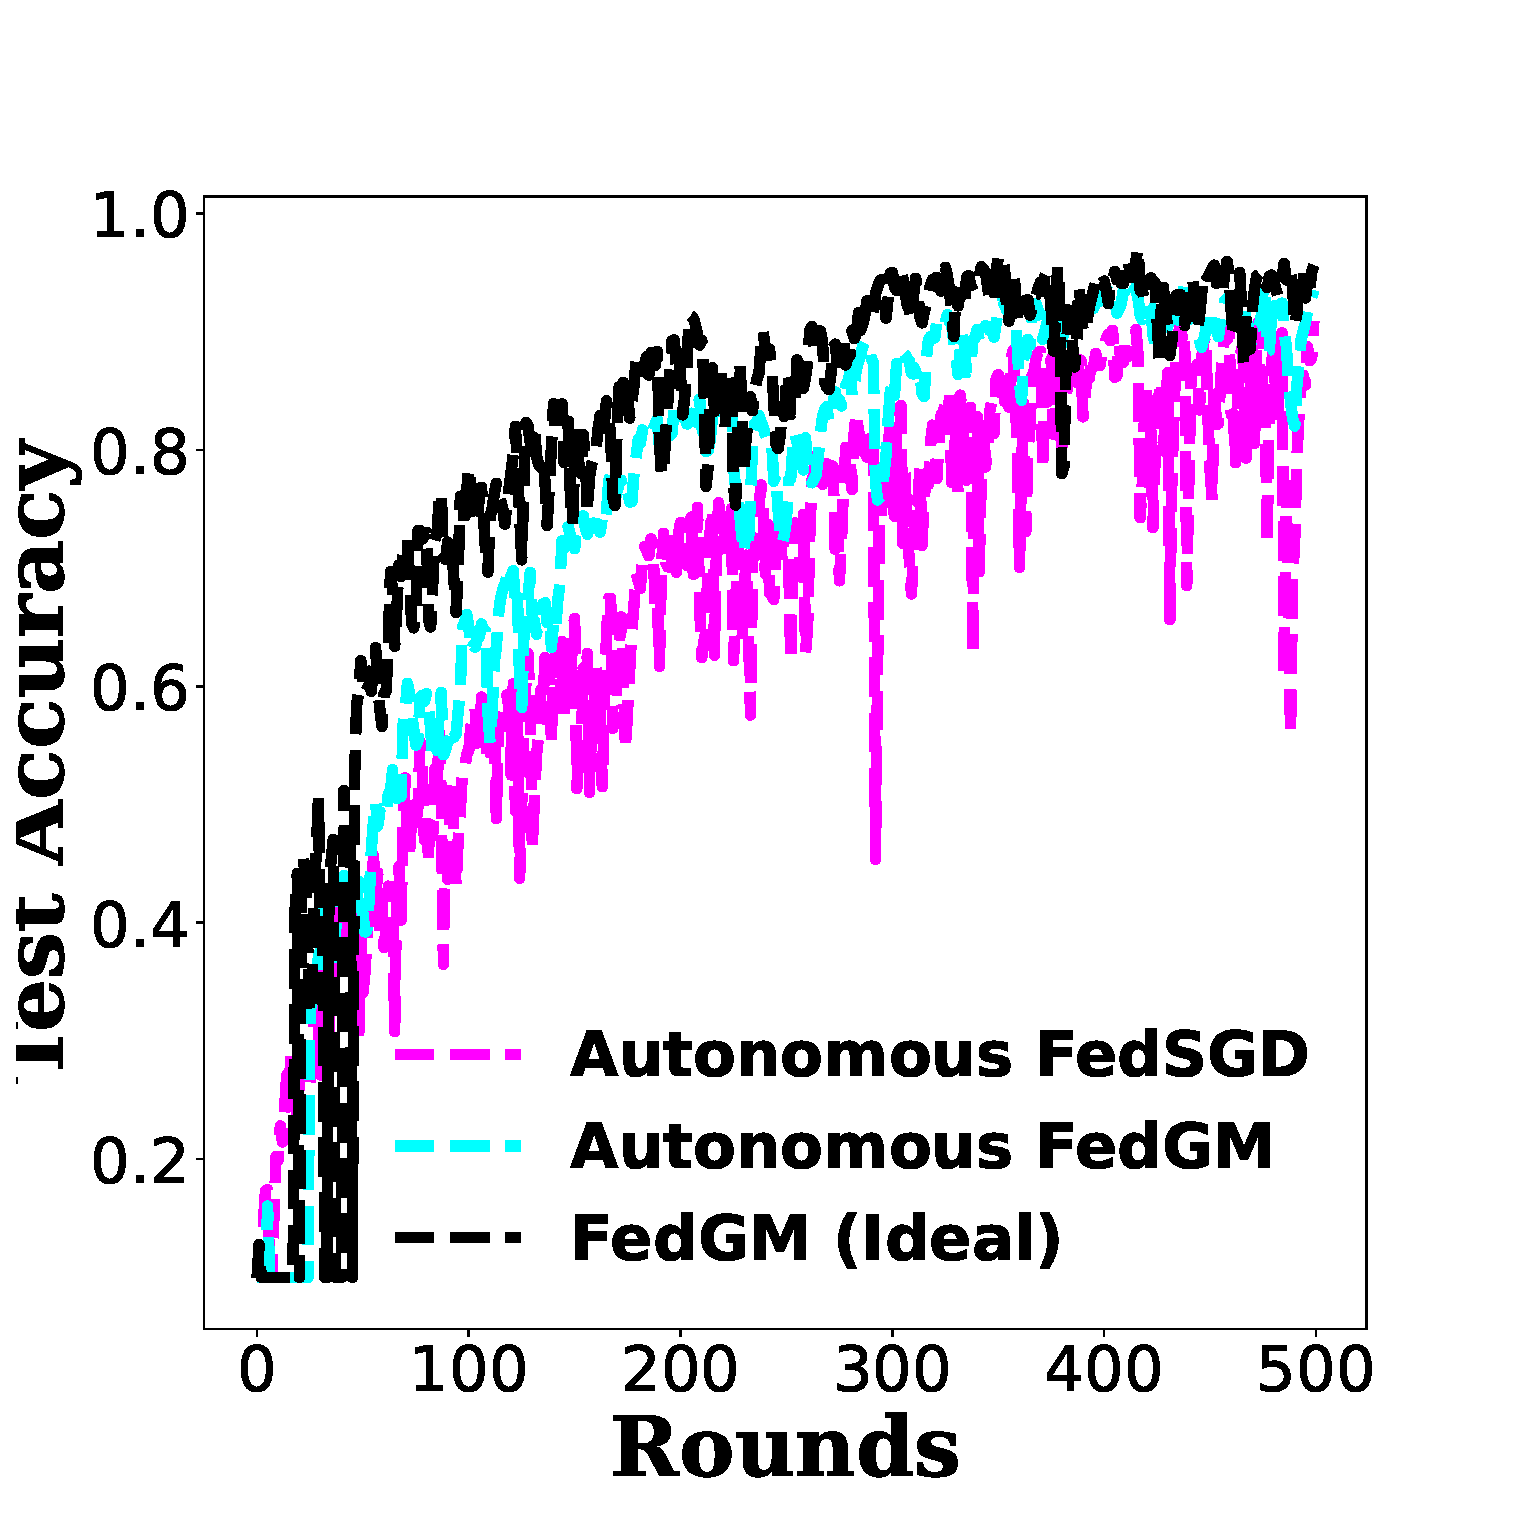
\includegraphics[width=.21\textwidth]{figs/autonomous_resnet_cifar10_train.eps}
\label{subfig:autonomous_resnet_cifar10_train}
}
\hspace{-2pt}
\subfigure{
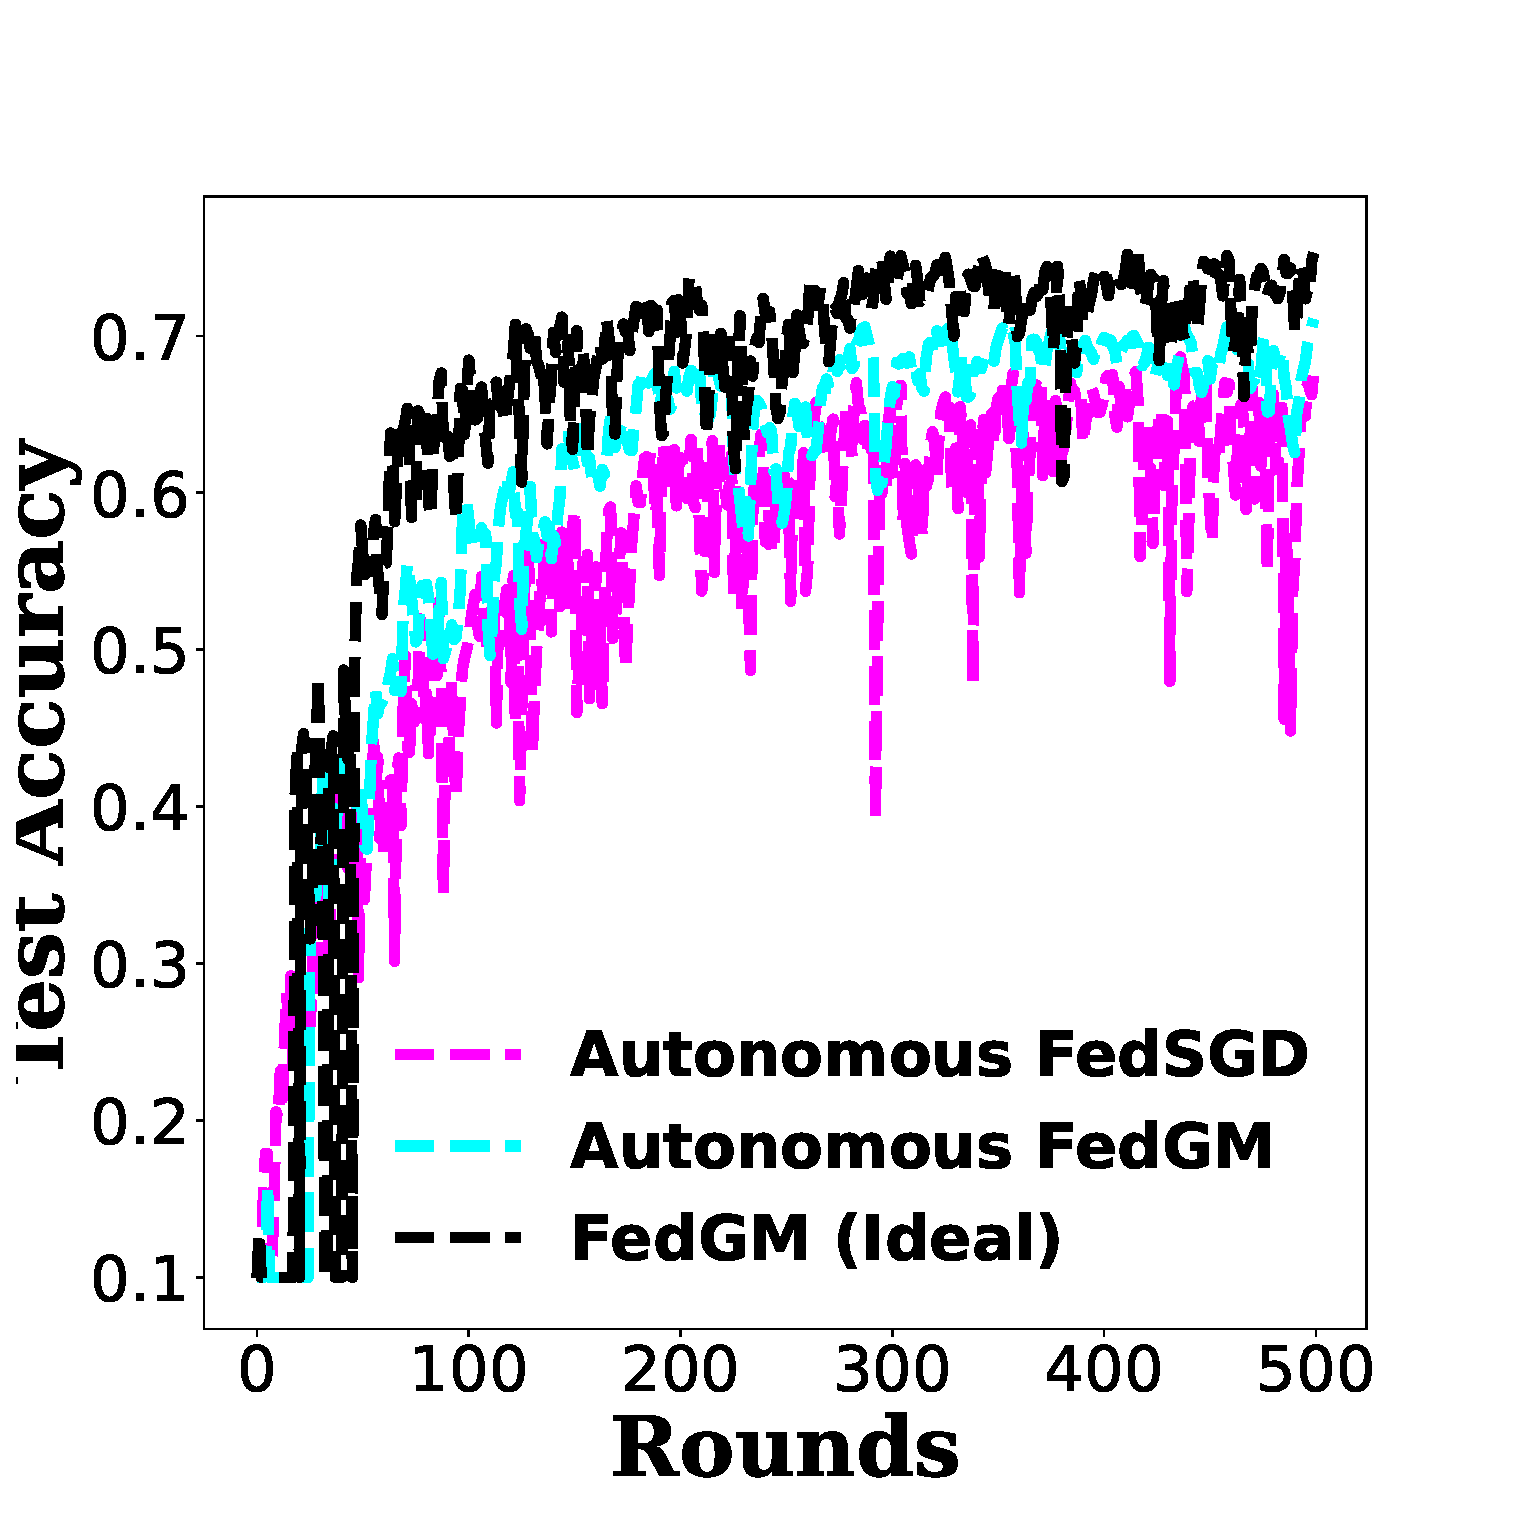
\includegraphics[width=.21\textwidth]{figs/autonomous_resnet_cifar10_test.eps}
\label{subfig:autonomous_resnet_cifar10_test}
}

\caption{\ref{subfig:resnet_cifar10_train} Training and \ref{subfig:resnet_cifar10_test} Testing Curves for FedGM (ResNet on CIFAR-10). FedGM outperforms FedAvg/FedAvgM. \ref{subfig:autonomous_resnet_cifar10_train} Training and \ref{subfig:autonomous_resnet_cifar10_test} Testing for Autonomous FedGM (ResNet on CIFAR-10).}
\label{fig:resnet_cifar10}

\end{figure}

\subsection{Convergence Analysis}

We state the convergence guarantee of autonomous multistage FedGM as follows,

\begin{theorem}
\label{multistage_fedgm_free_uniform_arrival_convergence_theorem}
We optimize $f(x)$ with Algorithm \ref{alg:autonomous_fedgm} under assumptions \ref{smoothness_assumption}-\ref{bounded_global_assumption}. Suppose the maximum delay is bounded, i.e. $\tau_{t,i}\leq\tau<\infty$ for any $i\in\mathcal{S}_t$ and $t\in\{0,1,\dots,T-1\}$. Under the condition $\eta_l\leq\min\left\{\frac{1}{8K_{t,\text{max}}L},\sqrt{\frac{1}{ 120L^2 C_\eta \tau K_{t,\text{max}}^2}} \right\}$, where $K_{t,\text{max}} =\max_{i\in\mathcal{S}_t}K_{t,i} $. And further assume each client is included in $\mathcal{S}_t$ with probability $\frac{m}{n}$ uniformly and independently. With necessary abbreviation for ease of notation \footnote{We denote $\Bar{\eta}\triangleq\frac{1}{S}\sum_{s=0}^{S-1}\eta_s$ (average server learning rate), $\hat{\eta}^2\triangleq\frac{1}{S}\sum_{s=0}^{S-1}\eta^2_s$, $\hat{\eta}^3\triangleq\frac{1}{S}\sum_{s=0}^{S-1}\eta^3_s$, $\frac{1}{K_t}=\frac{1}{m}\sum_{i\in\mathcal{S}_t}\frac{1}{K_{t,i}}$, $\bar{K}_t\triangleq \frac{1}{m}\sum_{i\in\mathcal{S}_t}K_{t,i}$, $\hat{K}_t^2 \triangleq \frac{1}{m}\sum_{i\in\mathcal{S}_t}K^2_{t,i}$, $\phi_1 \triangleq  \frac{1}{T}\sum_{t=0}^{T-1} \Bar{K}_t$, $\phi_2 \triangleq  \frac{1}{T}\sum_{t=0}^{T-1} \hat{K}_t^2$, and $\phi_3 \triangleq \frac{1}{T}\sum_{t=0}^{T-1} \frac{1}{K_t}$, for ease of notation.}, we would have:

\begin{gather*}
 \Bar{\mathcal{G}}
\leq \frac{4 \left(f(x_0) - f^\ast  \right)}{S W_2 \eta_l} 
+  \Phi_l \sigma_l^2
+ \Phi_g \sigma_g^2 
\label{multistage_fedgm_free_uniform_arrival_bound}
\end{gather*}
$\Phi_l \triangleq \frac{20  \eta^2_l L^2 T \Bar{\eta}}{W_2} \phi_1 + \frac{4 L^2\tau^2\hat{\eta}^3\eta_l^2T}{mW_2}\phi_3 + \frac{2 L^2W_1^2 \Bar{\eta} \eta_l T}{m W_2}\phi_3 + \frac{2 \Bar{\eta} \eta_l T}{m W_2}\phi_3 + \frac{2 L\hat{\eta}^2\eta_l}{m W_2}\phi_3$, and $\Phi_g \triangleq \frac{120 \eta^2_l L^2 T \Bar{\eta} \phi_2}{W_2}$. 
\end{theorem}



\begin{corollary}[Convergence Rate]
Suppose an identical $K$ for all $t$ and $i$. By appropriately setting $\Bar{\eta}$, $\eta_l$, $W_1$, $W_2$, we have the convergence rate as, $\mathcal{O}\left(\frac{1}{\sqrt{mKT}}\right)+ \mathcal{O}\left(\frac{\tau^2}{T}\right) +  \mathcal{O}\left( \frac{K^2}{T} \right)$.
\label{corollary:free_multistage_fedgm_rate}
\end{corollary}


\begin{remark}
Corollary \ref{corollary:free_multistage_fedgm_rate} indicates $\tau$ brings a slowdown in convergence. Fortunately, with a sufficiently large $T$ (e.g. $T\ge mK^5$) and a manageable $\tau$ (e.g. $\tau \leq \frac{T^\frac{1}{4}}{(mK)^\frac{1}{4}}$), autonomous multistage FedGM obtains a $\mathcal{O}\left(\frac{1}{\sqrt{mKT}}\right)$ rate. Note that we make an additional assumption that each client is included in $\mathcal{S}_t$ with probability $\frac{m}{n}$ uniformly and independently, which is necessary as the following Corollary \ref{corollary:free_multistage_fedgm_general_arrival_rate} indicates if without such assumption, the rate has a non-convergent $\mathcal{O}\left( \sigma_g^2 \right)$ term that we cannot avoid (the lower bound is $\Omega\left( \sigma_g^2 \right)$).
\end{remark}

\begin{corollary}[Convergence Rate w/o Uniform Sampling Assumption]
Suppose an identical $K$ for all $t$ and $i$. By appropriately setting $\Bar{\eta}$, $\eta_l$, $W_1$, $W_2$, we have the convergence rate as, $\mathcal{O}\left(\frac{1}{\sqrt{mKT}}\right)+ \mathcal{O}\left(\frac{\tau^2}{T}\right) +  \mathcal{O}\left( \frac{K^2}{T} \right) + \mathcal{O}\left( \sigma_g^2 \right)$, and the non-vanishing $\mathcal{O}\left( \sigma_g^2 \right)$ is unavoidable. \footnote{We informally state Corollary \ref{corollary:free_multistage_fedgm_general_arrival_rate} due to page limit, please refer to Appendix \ref{sec:proof_free_multistage_fedgm_general_arrival} for a formal statement.}
\label{corollary:free_multistage_fedgm_general_arrival_rate}
\end{corollary}




